\subsection{Standards Committees}
An important activity for ECP ST staff is participation in standards efforts.  In many instances, our software will not be sustainable if it is not tightly connected to a standard.  At the same time, any standard has to take into account the emerging requirements that Exascale platforms need in order to achieve performance and portability.  Figure~\ref{fig:standards} summarized ECP ST staff involvement in the major standards efforts that impact ECP.

ECP ST staff are heavily involved in MPI and OpenMP standards efforts.  ECP ST staff hold several key leadership positions and have heavy involvement in all aspects. ECP ST staff also play a critical role in C++ standards efforts.  While DOE staff have only recently engaged in C++ standards, our efforts are essential to  getting HPC requirements considered, especially by contributing working code that demonstrates requirements and design. ECP ST sponsors the newest open source Fortran compiler Flang~\ref{subsubsect:flang}, a front end for LLVM.  This compiler is a rapidly emerging and essential part of the HPC ecosystem.  In particular, while ARM processors are not explicitly part of the pre-Exascale ecosystem, they are emerging as a strong contender in the future.  Flang is \textit{the} Fortran compiler for ARM-based systems.  ECP ST involvement in other committees, including the \textit{de facto} also provide valuable leverage and improved uniformity for HPC software.  Lastly, we mention the Visualization Toolkit (VTK) Architecture Review Board (ARB).  While this is only a single instance, we intend to explore the ARB model as part of our SDK efforts.
\begin{figure}[htb]
	\begin{center}
		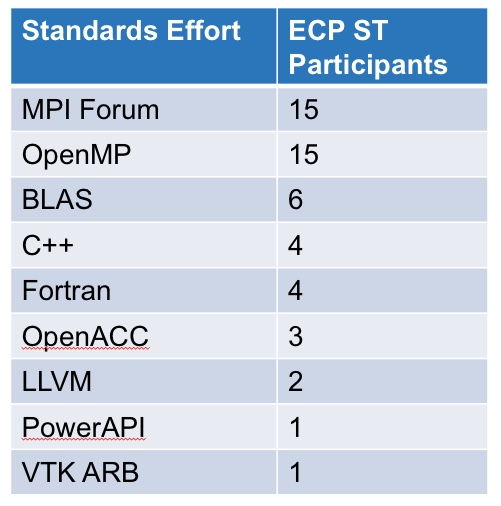
\includegraphics[width=0.5\textwidth]{StandardsInvolvement}
		
		\caption{\label{fig:standards} ECP ST staff are involved in a variety of official and \textit{de facto} standards committees.  Involvement in standards efforts is essential to assuring the sustainability of our products and to assure that emerging Exascale requirements are addressed by these standards.}
	\end{center}
\end{figure}
